\documentclass[11pt,a4paper,english]{article}
\usepackage[english]{babel} % Using babel for hyphenation
\usepackage{lmodern} % Changing the font
\usepackage[utf8]{inputenc}
\usepackage[T1]{fontenc}

\usepackage[colorlinks=true]{hyperref}

%\usepackage[moderate]{savetrees} % [subtle/moderate/extreme] really compact writing
\usepackage{tcolorbox}
\tcbuselibrary{hooks}
\usepackage[parfill]{parskip} % Removes indents
\usepackage{amsmath} % Environment, symbols etc...
\usepackage{amssymb}
\usepackage{float} % Fixing figure locations
\usepackage{multirow} % For nice tables
%\usepackage{wasysym} % Astrological symbols
\usepackage{graphicx} % For pictures etc...
\usepackage{enumitem} % Points/lists
\usepackage{physics} % Typesetting of mathematical physics examples: 
                     % \bra{}, \ket{}, expval{}
\usepackage{url}

\definecolor{red}{RGB}{255,10,10}

% To include code(-snippets) with æøå
\usepackage{listings}
\lstset{
language=c++,
showspaces=false,
showstringspaces=false,
frame=l,
}

\tolerance = 5000 % Bedre tekst
\hbadness = \tolerance
\pretolerance = 2000

\numberwithin{equation}{section}

\newcommand{\conj}[1]{#1^*}
\newcommand{\ve}[1]{\mathbf{#1}} % Vektorer i bold
\let\oldhat\hat
\renewcommand{\hat}[1]{\oldhat{#1}}
\newcommand{\trans}[1]{#1^\top}
\newcommand{\herm}[1]{#1^\dagger}

\newcommand{\Real}{\mathbb{R}}
\newcommand{\bigO}[1]{\mathcal{O}\left( #1 \right)}

\newcommand{\di}{\mathrm{d}}

\newcounter{algcounter}
\renewcommand{\thealgcounter}{\Roman{algcounter}}

\newenvironment{algorithm}{%
\refstepcounter{algcounter}
\begin{tcolorbox}
\centerline{Algorithm \thealgcounter}\vspace{2mm}
}
{\end{tcolorbox}}

\newcommand{\figurewidth}{.85\textwidth}

\title{FYS3150/4150\\Computational Physics\\Project 4}
\author{Candidate numbers ?? and ??}
\date{\today}

\begin{document}
\tcbset{before app=\parfillskip0pt}
\maketitle

\begin{abstract}
This project explores the Ising model applied to spins in two dimensions.
\end{abstract}



\section{Introduction}


\section{Theory}

The energy of a spin system in the Ising model 
\begin{gather}
E = -J\sum_{\expval{kl}}^N s_k s_l
\end{gather}
With $s_i = \pm 1$, N number of spins, J coupling constant, summed over 
the closest neighbours only. This leads to a boundary problem, which 
can be solved in multiple ways. In our model we are 
using periodic boundary conditions,
\begin{gather}
s_k = s_{k \pm L}
\label{eq:boundary}
\end{gather}
An illustration of this is visible in figure \ref{fig:spin_neighbours}.

\begin{figure}[H]
\centering
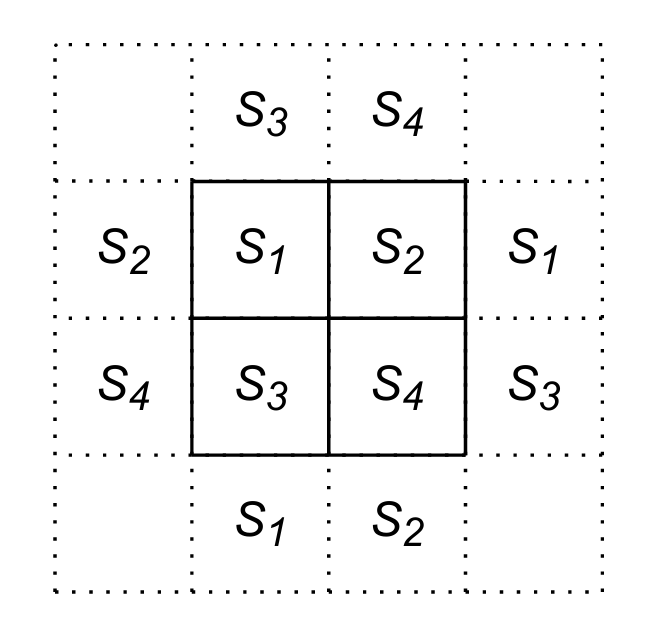
\includegraphics[scale=0.15]{pics/simple_lattice.png}
\caption{ Illustration of the simple, ''$L=2$''-lattice and a graphical interpretation the periodic boundary conditions.}
\label{fig:spin_neighbours}
\end{figure}





\subsection{Statistical mechanics}
The partition function
\begin{gather}
Z = \sum_i \exp(-\beta E_i)
\end{gather}

\subsubsection{Magnetisation}

The net magnetisation is defined by
\begin{gather}
\expval{M} = \sum_k s_k
\end{gather}
There should be a critical temperature where this one flips from 
zero to some value for ferromagnets (positive J)


\subsection{Simple system}
For the simple case of only two spins in each dimension($L=2$) the energies are:
\begin{align*}
E_1 = -J\sum_{<1l>}^{N}s_1 s_l = -J[2(s_1 s_2)+2(s_1 s_3)] \\
E_2 = -J\sum_{<2l>}^{N}s_2 s_l = -J[2(s_2 s_1)+2(s_2 s_4)] \\
E_3 = -J\sum_{<3l>}^{N}s_3 s_l = -J[2(s_3 s_1)+2(s_3 s_4)] \\
E_4 = -J\sum_{<4l>}^{N}s_4 s_l = -J[2(s_4 s_2)+2(s_4 s_3)] 
\end{align*}
And the total energy for a state 
\begin{equation}
E = -4J(s_1s_2 + s_1s_3 + s_1s_4 + s_2s_3 + s_2s_4 + s_3s_4)
\end{equation}
Which seems very symmetric. Listing up all the different energies,
with degeneracy
\begin{gather*}
 E = 
\begin{cases}
-24J,\,\,n_{up} = 0,\quad d = 1\\
-8J,\quad n_{up} = 1,\quad d = 4\\
\phantom{-}4J, \quad n_{up} = 2, \quad d = 6\\
-8J,\quad n_{up} = 3, \quad d= 4\\
-24J,\,\,\,n_{up} = 4, \quad d = 1
\end{cases}
\end{gather*}

Now to find the partition function and calculate all the properties,

\subsection{Analytical solutions}

\textcolor{red}{KSK: Maybe make this section consistent with the notation of $\beta = 1/ k_B T$ ? And add reference for 2D. solution}

\subsubsection{1-D Ising model}
Solutions for the Ising model in one dimension for a very large number of particles are known(Plischke and Bergersen, 1994). 

\begin{equation}
\frac{U}{J} = -N tanh \left( \frac{J}{k_B T} \right) = -N \frac{e^{J/k_B T}-e^{-J/k_B T} }{e^{J/k_B T}+ e^{-J/k_B T} } =  \begin{cases} N, \quad k_B T \to 0 \\ 0, \quad  k_B T \to \infty \end{cases}
\end{equation}

The specific heat per particle and the magnetization are given by 

\begin{equation}
C(T) = \frac{1}{N} \frac{dU}{dT} = \frac{(J/k_B T)^2}{cosh^2 (J/k_B T)}
\end{equation}
\begin{equation}
M(T) = \frac{N e^{J / k_B T} sinh(B/k_B T) }{ \sqrt{ e^{2J/k_B T} sinh^2 (B/k_B T) + e^{-2J/ k_B T}  } }
\end{equation}

\subsubsection{2-D Ising model}
There are known analytical solution to the two dimensional model as well, 

\begin{equation}
\mathcal{M}(T) = \begin{cases} 0, \quad T > T_C \\ \frac{(1+z^2)^{1/4} (1-6z^2 + z^4 )^{1/8} }{(1-z^2)^{1/2}}, \quad T < T_C \end{cases}
\end{equation}
\begin{equation}
k T_C/J = \frac{2}{ln(1+ \sqrt{2}) } \approx 2.269
\end{equation}

here $T_C$ is the \emph{Curie temperature} and $z = e^{-2J/k_B T}$. 

\section{Implementation}

A lattice class with periodic boundary conditions, so access of an
element follows \eqref{eq:boundary}. The energy of an element in the 
lattice and the total energy is easily calculated from the definition
of the energy. 

\subsection{The metropolis algorithm}

The probability of transition from i to j 
is modelled by the Boltzmann coefficient
\begin{gather}
w_j = \exp(-\beta (E_i - E_j))
\end{gather}
This suggest the following probabilities for moving to this state:
\begin{gather}
p = \begin{cases}
1 \quad\text{ if }  E_i - E_j \le 0\\
\exp(-\beta \Delta E) \text{ else}
\end{cases}
\label{eq:transition}
\end{gather}
This probability is compared with a random number generated from 
the computer.

For our lattices the factor $\Delta E$ is rather simple. Considering 
a case with one spin $s_0$ surrounded by $s_1,s_2,s_3, s_4$. 

\textcolor{red}{MU: Could you please make a figure like \ref{fig:spin_neighbours}
for this case? Thanks!}

This gives a flip of spin $s_0$ results in a n
energy-difference of the lattice which is
is -3 times the energy of $s_0$.
\begin{gather}
\Delta E = -4s_0(s_1 + s_2 + s_3 + s_4)
\end{gather}
It is also clear that this is quantized, which means that the 
exponential function in \eqref{eq:transition} can be precomputed.
\begin{gather}
\Delta E \in \{16, 8, 0, -8, -16\}
\end{gather}




\subsubsection{Choice of random number generator}
The pseudo random number generator used for the simulations covered in 
this report is the Mersenne Twister engine
instantated with the parameters of 
\emph{Mersene Twister 19937 generator} seeded with the time.
This is available in the \texttt{<random>} header of the standard
library in \emph{C++} and has a period of the \emph{mersenne number}, $2^{(n-1)w}-1$.
The instatation chosen gives $w=32$ and $n=624$.	

\subsection{Test environment}

The testing framework is \href{https://github.com/philsquared/Catch}{Catch}.
The testcases should be self-explanatory.


\section{Results}

\subsection{Reproduction of results}

To see benchmark calculations along with programs used see:\\
\url{https://github.com/mulimoen/FYS3150CompPhy/}\\
Under the folder \emph{Project 4}.

\section{Conclusion}

\section{Refrences}



\end{document}